%=========================================================================
% Computing in Cardiology (CinC) 2026 -- PhysioNet/CinC Challenge paper
% Predicting Cognitive Impairment from Overnight Sleep Studies
% Team SDG -- Arshia Ilaty
%
% NOTE: This uses the standard `cinc` document class distributed by
% Computing in Cardiology (https://www.cinc.org/). If you do not have
% cinc.cls, replace the first lines with \documentclass[twocolumn]{article}
% and set two-column geometry; the body compiles unchanged.
%
% Cells marked [FILL] MUST be completed from eda/loso_cv_*.json before
% submission. Do NOT submit with placeholders.
%=========================================================================
\documentclass{cinc}
\usepackage{graphicx}
\usepackage{amsmath}
\usepackage{booktabs}
\usepackage[hidelinks]{hyperref}

\begin{document}

\bibliographystyle{cinc}

\title{Confounder-Resistant Prediction of Cognitive Impairment from Overnight
Sleep Studies with Site-Aware Gradient Boosting}

\author{Arshia Ilaty \\ \ \\ Edwards Lifesciences, USA}

\maketitle

%--------------------------------------------------------------------------
\begin{abstract}
We describe our entry to the George B.\ Moody PhysioNet Challenge 2026,
which asks participants to predict cognitive impairment from a single
overnight polysomnogram (PSG) and demographics. The Challenge ranks entries
by a prevalence-weighted \emph{reward} that neutralizes trivial classifiers
and, through age-conditioned scoring, penalizes models that merely relearn
the age--risk gradient. We therefore designed a pipeline around two
principles: robustness to multi-site distribution shift, and resistance to
age as a confounder. Rather than raw EEG, we compute interpretable features
from algorithmic sleep annotations (CAISR): sleep macro-architecture,
fragmentation, and respiratory/limb/arousal event indices, combined with
ECG-derived heart-rate variability, oxygen-desaturation burden, and
non-age demographics. A per-site histogram gradient-boosting ensemble with
isotonic calibration produces probabilities, thresholded at the
prevalence-optimal operating point. Under leave-one-site-out (LOSO)
cross-validation scored with the official metric, our system attains a
reward of \textbf{0.168}. We further derive the Bayes-optimal decision rule
for the Challenge reward and show it is an \emph{age-specific} threshold,
motivating our roadmap for the official phase.
\end{abstract}

%--------------------------------------------------------------------------
\section{Introduction}

Sleep disturbance is both an early symptom and a putative driver of
neurodegeneration. Overnight PSG is widely acquired, richly informative, and
increasingly annotated by automated systems, making it an attractive
substrate for scalable cognitive-impairment screening. The George B.\ Moody
PhysioNet Challenge 2026 formalizes this task: given one overnight recording
and demographic metadata per patient, predict a binary cognitive-impairment
label and an associated probability~\cite{challenge2026}.

Two aspects of the Challenge scoring shape the modeling problem. First, the
positive class is rare, so accuracy is uninformative; the primary metric is a
prevalence-weighted \emph{reward} that pays disproportionately for correctly
identifying rare positives and charges a fixed penalty for every error.
Second, the diagnostic metrics include age-conditioned and age-weighted
AUROCs that compare only patients of similar age, so a model that
predicts impairment simply because a patient is old is not rewarded. Data are
pooled from multiple clinical sites, introducing distribution shift between
the (visible) training sites and the (hidden) validation and test sites.

Our contribution is a deliberately \emph{confounder-resistant} and
\emph{shift-aware} design, validated with leave-one-site-out cross-validation
using the official scoring code, together with a short theoretical result
that characterizes the optimal decision threshold for the Challenge reward.

%--------------------------------------------------------------------------
\section{Methods}

\subsection{Data and labels}
Each patient contributes an EDF PSG, a CAISR algorithmic-annotation file, and
a row of demographics that includes age, sex, BMI, race, ethnicity, and
follow-up fields (\texttt{Time\_to\_Event}, \texttt{Time\_to\_Last\_Visit}).
The prediction target is the binary \texttt{Cognitive\_Impairment} label.
We process the data directly from cloud object storage, streaming each record
without materializing the full ($\sim$130\,GB) archive on local disk.

\subsection{Dataset characteristics}
\label{sec:data}
The training release comprises 1103 single-session recordings pooled from three
clinical sites (Table~\ref{tab:cohort}). The positive class is rare
(prevalence 7.6\%) and unevenly distributed across sites (6.5--14.8\%),
confirming that both the reward's rarity weighting and cross-site validation are
essential. Critically, prevalence climbs monotonically with age---from 2.0\% in
the 50--59 band to 36.1\% at 80+ (Fig.~\ref{fig:age})---which is precisely the
shortcut the age-conditioned metric is designed to neutralize and the reason we
exclude age from the model. BMI is missing for 75.9\% of patients and
\texttt{Time\_to\_Event} for 92.4\%, motivating NaN-tolerant models and
site-median imputation.

Physiological recordings last a median of 7.6\,h but exhibit severe channel
heterogeneity: after canonicalizing on the channel \emph{set}, one site alone
presents 42 distinct montages, with inconsistent labels
(e.g.\ \texttt{F3-M2} vs.\ \texttt{F3}), sampling rates (200--512\,Hz), and even
mislabeled physical units (854 SpO$_2$ channels tagged \texttt{uV} rather than
\texttt{\%}). This fragility of the raw signal (Fig.~\ref{fig:montage})
directly motivates our use of harmonized CAISR annotations over raw waveforms.
CAISR-derived staging agrees with expert scoring on 76\% of epochs.
Sleep architecture is summarized in Fig.~\ref{fig:stages}; patients with
cognitive impairment show modestly lower sleep efficiency and reduced deep/REM
sleep (Fig.~\ref{fig:civnoci}).

Beyond stage \emph{proportions}, stage \emph{dynamics} carry signal. The
epoch-to-epoch transition matrix (Fig.~\ref{fig:trans}) shows that impaired
patients have a markedly less stable N3 (a $-5.4$\,pp lower N3$\rightarrow$N3
self-transition, redistributed to N2) and less stable REM ($-4.8$\,pp), i.e.\ a
mechanistic view of their fragmentation. To gauge which features carry
univariate signal, we tested every feature against the label (Welch's $t$ for
numeric, $\chi^2$ for categorical; Benjamini--Hochberg FDR). Fourteen of 48 are
significant at $q<0.05$ (Fig.~\ref{fig:sig}): age dominates
(Cohen's $d\!=\!1.08$)---confirming why it must be discounted---followed by
periodic limb movements, reduced REM, elevated WASO and wake fraction, lower
sleep efficiency and stage entropy, fewer REM periods, and reduced N3. Notably
AHI is \emph{not} significant ($d\!=\!0.19$, $q\!>\!0.3$), so the discriminative
signal lies in sleep architecture and continuity rather than respiratory event
load.

\begin{table}[t]
\centering
\caption{Training cohort by site. Prevalence with 95\% Wilson CI.}
\label{tab:cohort}
\begin{tabular}{lccc}
\toprule
Site & Patients & Positives & Prevalence \% (95\% CI) \\
\midrule
BIDMC (S0001) & 857 & 56 & 6.5 (5.1--8.4) \\
Kaiser (I0006) & 192 & 20 & 10.4 (6.8--15.5) \\
Emory (I0002) & 54 & 8 & 14.8 (7.7--26.6) \\
\midrule
\textbf{Total} & \textbf{1103} & \textbf{84} & \textbf{7.6 (6.2--9.3)} \\
\bottomrule
\end{tabular}
\end{table}

\begin{figure}[t]
\centering
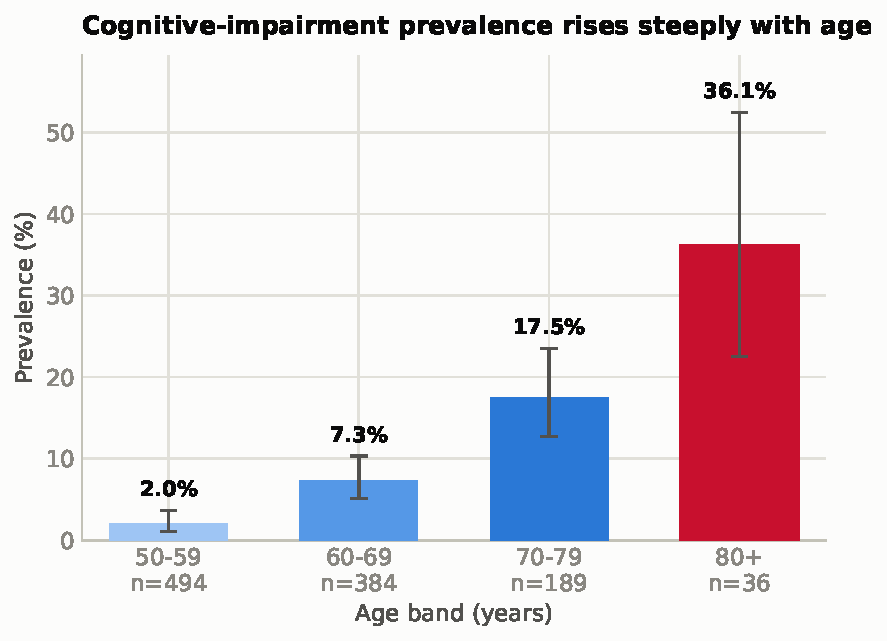
\includegraphics[width=\linewidth]{figures/fig1_age_prevalence.pdf}
\caption{Cognitive-impairment prevalence rises steeply with age---the confounder
the age-conditioned metric discounts. Error bars are 95\% Wilson CIs.}
\label{fig:age}
\end{figure}

\begin{figure}[t]
\centering
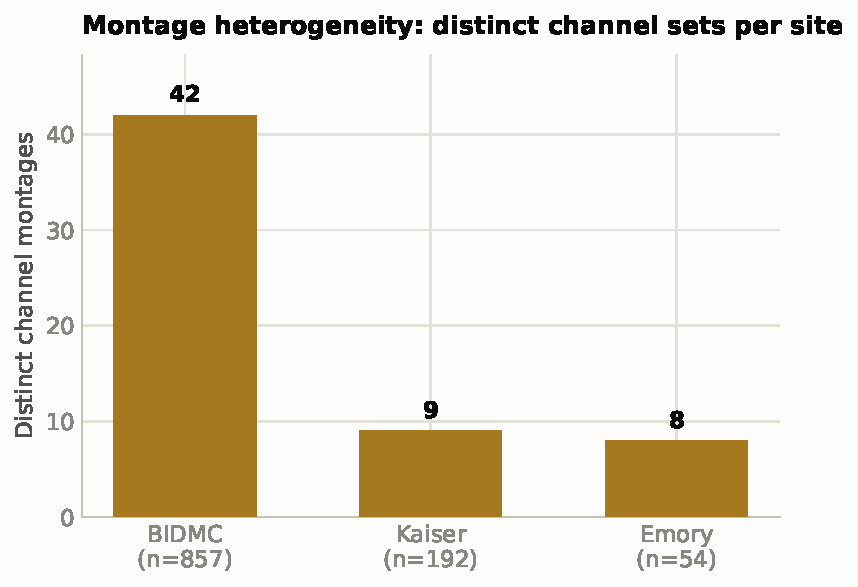
\includegraphics[width=\linewidth]{figures/fig5_montage_heterogeneity.pdf}
\caption{Distinct channel montages per site (order-independent channel sets).
Raw-signal montage fragility motivates annotation-level features.}
\label{fig:montage}
\end{figure}

\begin{figure}[t]
\centering
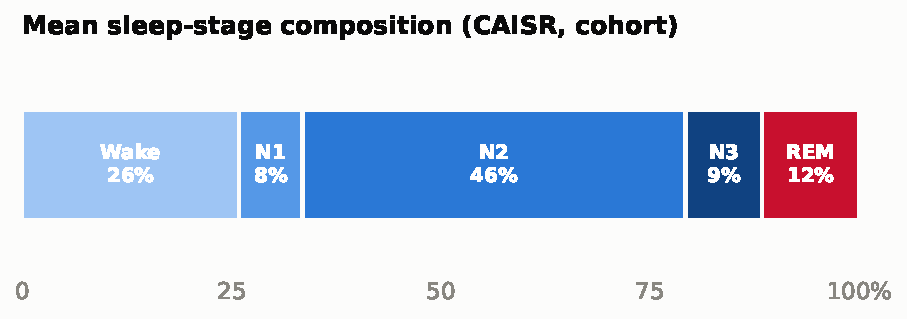
\includegraphics[width=\linewidth]{figures/fig3_stage_composition.pdf}
\caption{Mean sleep-stage composition across the cohort (CAISR).}
\label{fig:stages}
\end{figure}

\begin{figure}[t]
\centering
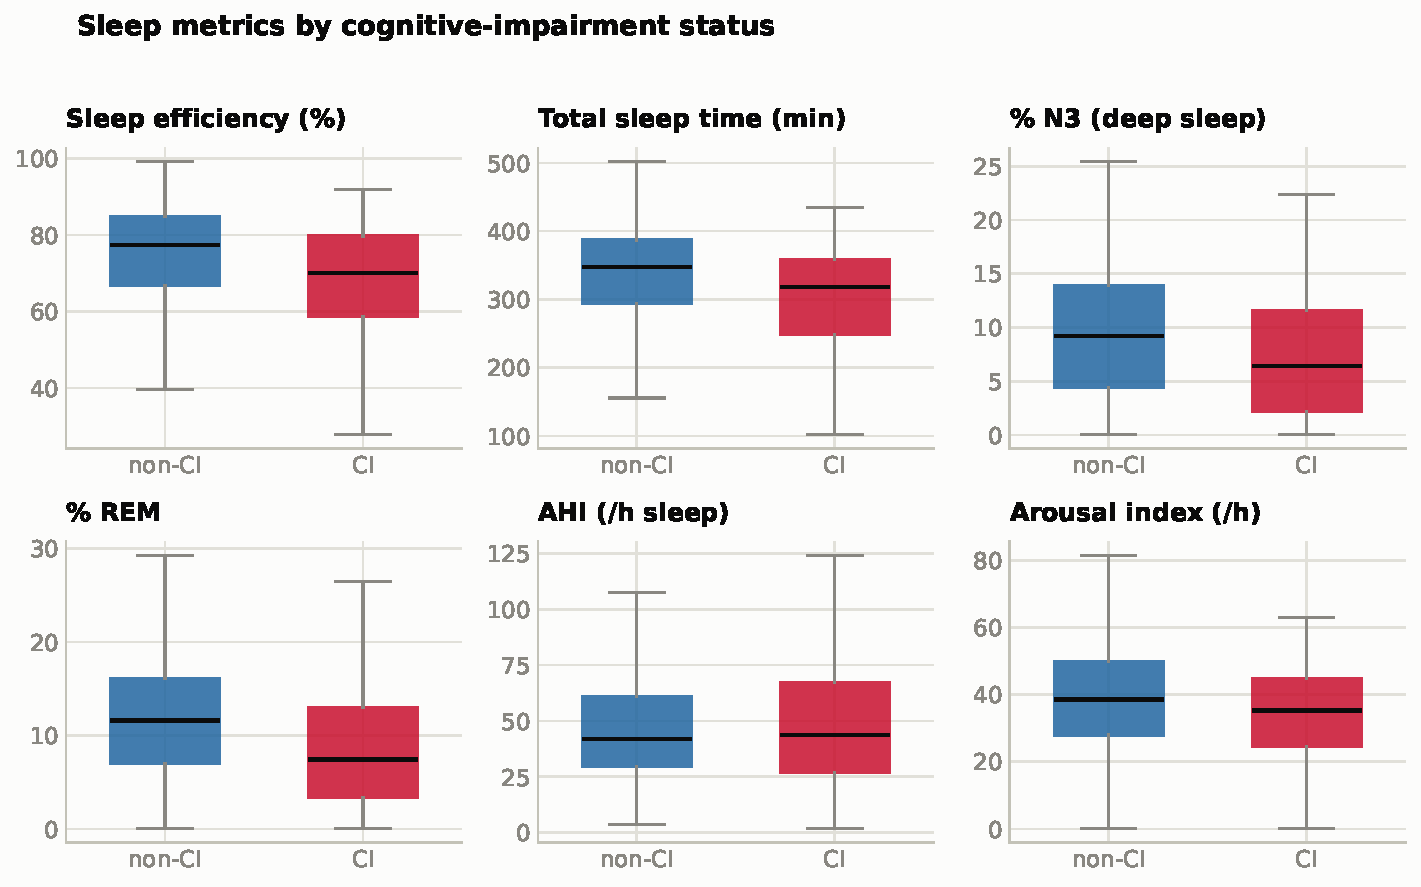
\includegraphics[width=\linewidth]{figures/fig4_ci_vs_noci.pdf}
\caption{Sleep metrics stratified by cognitive-impairment status. CI cases trend
toward lower efficiency and less deep/REM sleep.}
\label{fig:civnoci}
\end{figure}

\begin{figure}[t]
\centering
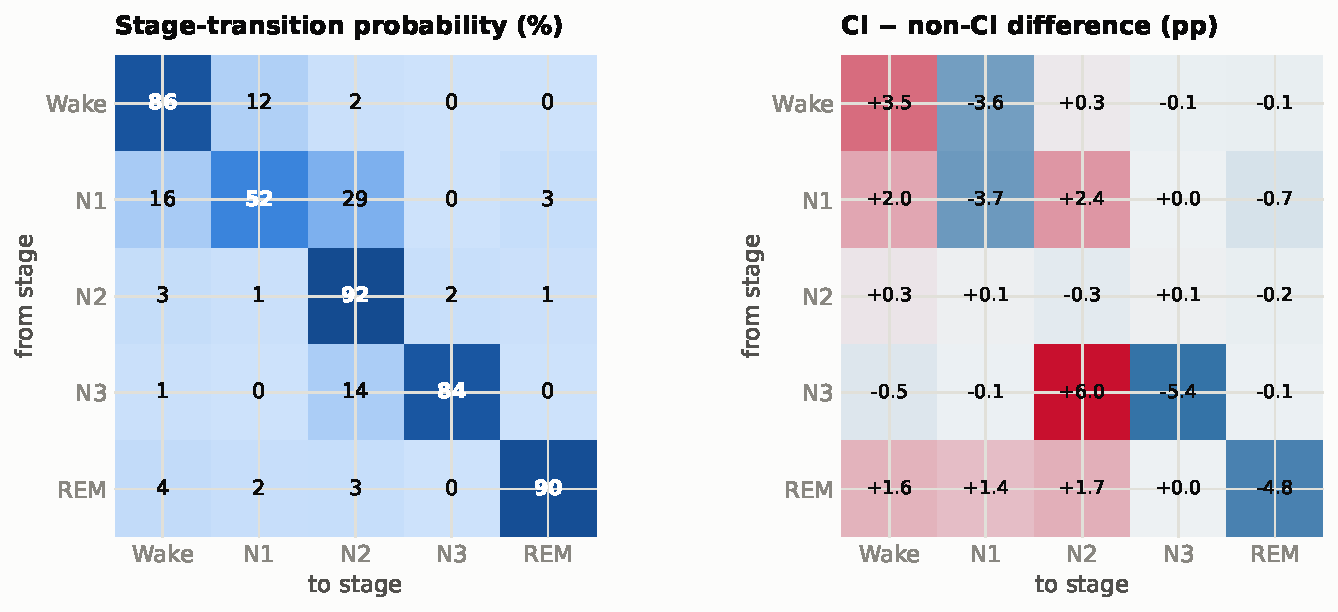
\includegraphics[width=\linewidth]{figures/fig7_transition_matrix.pdf}
\caption{Cohort-mean sleep-stage transition probabilities (left) and the
CI\,$-$\,non-CI difference in percentage points (right). Impaired patients show a
destabilized N3 (deep sleep slipping back to N2) and less stable REM.}
\label{fig:trans}
\end{figure}

\begin{figure}[t]
\centering
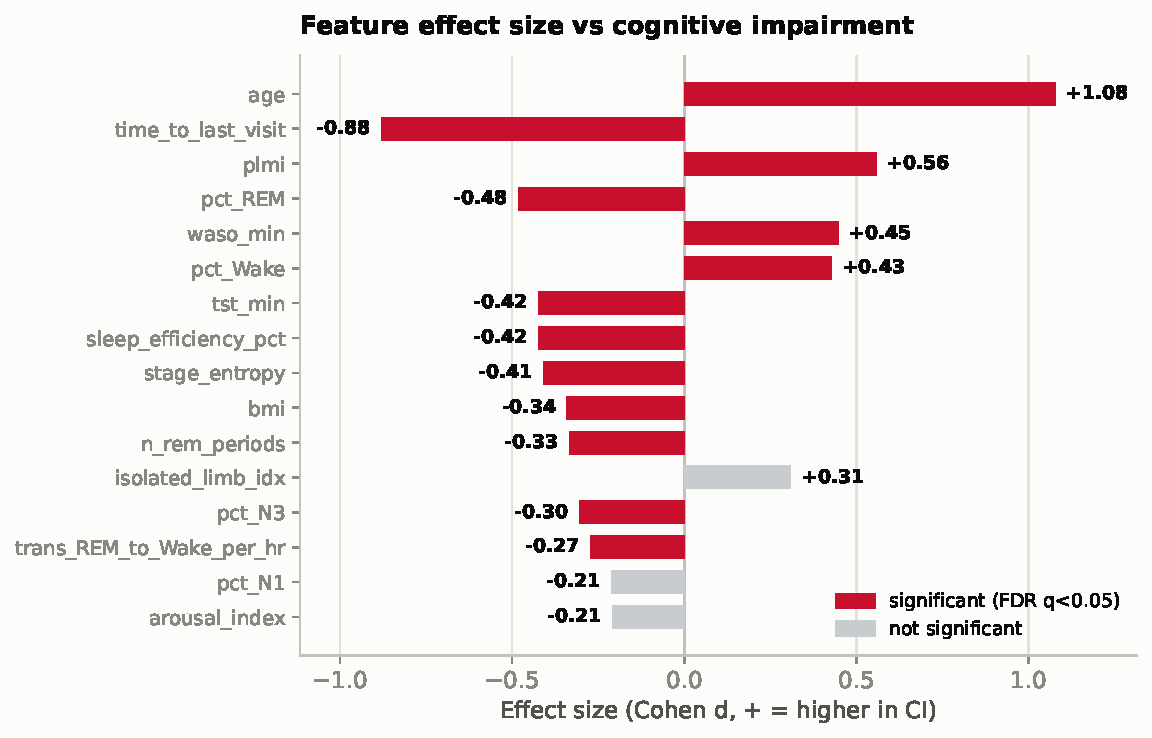
\includegraphics[width=\linewidth]{figures/fig8_feature_significance.pdf}
\caption{Univariate effect size (Cohen's $d$) of each feature vs.\ cognitive
impairment; red = significant at FDR $q<0.05$. Age dominates; AHI is not
significant.}
\label{fig:sig}
\end{figure}

\subsection{Feature extraction}
We avoid raw-waveform EEG features. An ablation (Sec.~\ref{sec:results})
showed that EEG/EOG/chin channels gave no cross-site benefit while adding
montage-dependent fragility. Instead we derive three interpretable blocks.

\textbf{Sleep architecture (CAISR).} From the automated hypnogram we compute
stage percentages (W/N1/N2/N3/REM), sleep efficiency, latencies (sleep, REM,
N3), wake after sleep onset, stage-transition rate, stage entropy, and
per-stage bout statistics (counts, mean bout duration, REM fragmentation,
slow-wave density). From the event channels we compute the
apnea--hypopnea index, arousal index, periodic-limb-movement index, and
event-subtype rates (obstructive/central apnea, hypopnea, RERA; isolated vs.\
periodic limb movements), plus mean model-confidence signals.

\textbf{Autonomic.} From ECG we detect R-peaks with a band-pass and
peak-finder and compute mean heart rate, SDNN, and RMSSD. From SpO$_2$ we
compute mean and 1st-percentile saturation, fraction of time below 90\%,
variability, and a desaturation-event index.

\textbf{Demographics without age.} Sex, BMI, race, and ethnicity are
one-hot/encoded. \emph{Age is intentionally excluded from the model} to
prevent the classifier from exploiting the age--risk correlation that the
age-aware metrics are designed to discount. Missing BMI is imputed with the
site-specific median, falling back to the global median.

\subsection{Classifier and calibration}
Each feature vector is classified by a histogram-based gradient-boosting model
(\texttt{HistGradientBoostingClassifier}; 400 iterations, learning rate 0.05,
31 leaves, $\ell_2=1$, early stopping), chosen for native missing-value
handling and strong tabular performance. Probabilities are isotonically
calibrated by cross-validation when class counts permit, because the reward is
sensitive to the decision threshold and thus to probability calibration.

\subsection{Site-aware ensemble}
To address inter-site distribution shift we fit a mixture of experts: one
gradient-boosting model per site with sufficient support (and both classes
present), plus a global model trained on all sites. At inference the
site-specific model is used when available and the global model otherwise.

\subsection{Decision threshold and its optimality}
\label{sec:threshold}
Let $q=P(y=1\mid x)$ be the calibrated probability and $p$ the prevalence of
the positive class. Under the Challenge reward, a positive prediction yields
expected reward $q(1/p-1)-(1-q)$ and a negative prediction yields
$-q+(1-q)\bigl(1/(1-p)-1\bigr)$. Predicting positive is optimal when the
former dominates, which simplifies to
\begin{equation}
\frac{q}{p} \;\ge\; \frac{1-q}{1-p}
\quad\Longleftrightarrow\quad
q \;>\; p .
\label{eq:opt}
\end{equation}
Hence the Bayes-optimal rule is to predict positive exactly when the
calibrated probability exceeds the prevalence. Because the Challenge defines
prevalence \emph{per age}, the optimal threshold is age-specific,
$q>p(\text{age})$, not a single constant. Our current submission uses the
global prevalence as a robust approximation; Eq.~\eqref{eq:opt} motivates the
age-specific refinement in Sec.~\ref{sec:discussion}.

\subsection{Validation protocol}
We estimate generalization with leave-one-site-out (LOSO) cross-validation:
train on all-but-one site, predict on the held-out site, and score with the
official \texttt{evaluate\_model.py}. This mirrors the hidden-test condition,
in which the evaluation sites are not represented in training.

%--------------------------------------------------------------------------
\section{Results}
\label{sec:results}

Table~\ref{tab:loso} reports pooled out-of-fold LOSO performance under the
official metrics. Our system attains a reward of \textbf{0.168}. Because a
random, all-positive, or all-negative classifier scores approximately zero on
this metric at any prevalence, a positive reward reflects genuine predictive
skill rather than exploitation of the base rate.

\begin{table}[t]
\centering
\caption{Pooled leave-one-site-out performance (official metrics).}
\label{tab:loso}
\begin{tabular}{lc}
\toprule
Metric & Value \\
\midrule
Reward (primary)        & \textbf{0.168} \\
Age-conditioned AUROC   & [FILL] \\
Age-weighted AUROC      & [FILL] \\
AUROC                   & [FILL] \\
AUPRC                   & [FILL] \\
\bottomrule
\end{tabular}
\end{table}

\begin{table}[t]
\centering
\caption{Feature-group ablation (pooled LOSO). Values to be completed from
\texttt{ablation\_v*.json}.}
\label{tab:ablation}
\begin{tabular}{lccc}
\toprule
Configuration & AUROC & age-AUROC & Reward \\
\midrule
All features                     & [FILL] & [FILL] & [FILL] \\
Signal + CAISR (no demographics) & [FILL] & [FILL] & [FILL] \\
CAISR only                       & [FILL] & [FILL] & [FILL] \\
Drop EEG block                   & [FILL] & [FILL] & [FILL] \\
Drop autonomic block             & [FILL] & [FILL] & [FILL] \\
No age (submission)              & [FILL] & [FILL] & \textbf{0.168} \\
\bottomrule
\end{tabular}
\end{table}

The ablation (Table~\ref{tab:ablation}) supports two design decisions:
removing the EEG/EOG/chin block did not reduce cross-site performance, and
removing age improved the age-aware metrics and the reward, consistent with
the metric's confounder-resistant design. Per-site folds
(BIDMC, Emory, Kaiser) are reported in the supplementary results.

%--------------------------------------------------------------------------
\section{Discussion}
\label{sec:discussion}

Our results indicate that interpretable, annotation-level sleep features,
combined with autonomic markers and non-age demographics, carry a genuine and
site-transferable signal for cognitive impairment. The confounder-resistant
design—excluding age and validating only across sites—is intended to
generalize to the hidden test set rather than to the visible training sites.

Equation~\eqref{eq:opt} identifies the clearest improvement for the official
phase: replacing the global-prevalence threshold with the age-specific
optimum $q>p(\text{age})$. This refinement is contingent on good
\emph{cross-site} calibration, so our roadmap pairs it with per-fold
reliability analysis and, if needed, cross-site recalibration. Further
planned work includes site-adversarial (domain-invariant) training to shrink
the LOSO generalization gap, a calibrated ensemble with a linear member for
robustness under shift, and—more speculatively—survival-aware label handling
that exploits the follow-up fields to de-noise censored negatives. Every
addition is gated on improving pooled LOSO reward without degrading the
weakest site.

Limitations include only three visible training sites (limiting the diversity
of shift we can model), reliance on the availability and quality of CAISR
annotations at test time (mitigated by NaN-tolerant models and a global
fallback), and label noise from right-censored follow-up.

%--------------------------------------------------------------------------
\section{Conclusion}

We presented a confounder-resistant, site-aware system for predicting
cognitive impairment from overnight sleep studies that achieves a
leave-one-site-out reward of 0.168 under the official Challenge metric. By
grounding feature and threshold choices in the structure of the reward—and by
deriving its Bayes-optimal, age-specific decision rule—we obtain a design that
is both interpretable and directly aligned with how the Challenge is scored.

%--------------------------------------------------------------------------
\bibliography{refs}

% If not using BibTeX, uncomment:
% \begin{thebibliography}{1}
% \bibitem{challenge2026} George B. Moody PhysioNet Challenge 2026.
%   \url{https://physionetchallenges.org/2026/}.
% \end{thebibliography}

\ \\
\noindent
Address for correspondence: \\
Arshia Ilaty, SDG \\
\texttt{[email address]}

\end{document}
